\section{Detectability Computation and Noise-Stress Protocol}
\label{sec:supp-theory}

\paragraph{Operators.} The information analysis of the main article uses
the nominal bank built by the evaluated implementation for one held-out
calibration record of a later campaign whose runtime is byte-identical to
the independent evaluation runtime. The independent-evaluation banks had
been evicted by the storage-retention policy; the nominal operators differ
between records only through the prefix-estimated operating factors, which
remain within $2\times10^{-5}$ of unity.

\paragraph{Signatures.} For each source $i$, the noise-free switched
predictor is propagated from a zero pre-event deviation with the ON
operator at half-phase 0 followed by the stay operator (loads at severity
0.1). Each candidate filter $j\in\{0,\dots,18\}$ is run on these reports with
the quiet-regime gains $K_o$ and inverse innovation covariances
$S_o^{-1}$ of the implementation. The cumulative sums
$\sum e^\top S^{-1}e$, $\sum s^\top S^{-1}e$ and $\sum s^\top S^{-1}s$ give the
signature information of the main article with the competitor's severity profiled
on $[-0.2,0.2]$. As a check, the true-history filter at the true severity
leaves a residual energy below $10^{-8}$. The idealized score reference uses the
birth hazard $1-\exp[-(1/60)/30]$ shared equally by the 18 cells.

\paragraph{Reset cost.} For every intervention of the controlled study,
the noise-free truth is propagated through ON, the active interval, OFF and
the gap until the next onset. At the inferred closure time of the carry
arm, the first 114 coordinates of the true augmented state are zeroed, and
the no-intervention and all birth filters are run on the remaining truth
in the recovery covariance regime. The largest profiled gain of a birth
over the no-intervention history is compared with the idealized score
reference $\lambda^\star$, not a publication guarantee. Harm in
the reset arm is an unmatched alarm between the OFF of the intervention and
the next onset, or a lost timely attribution of the next intervention.

\paragraph{Noise stress.} Observations are regenerated from the stored
deterministic trajectories with the simulator's own noise stream and seed:
$\varepsilon=c+\alpha(v-c)$ for multiplier $\alpha$, where $v$ is the stream
and $c$ its normalization center, exactly as the campaign exporter. The
$\alpha=1$ observations reproduce the original files to $6\times10^{-10}$
and the inference reproduces all 18 published messages of the parity
record. The independent-noise scenarios add zero-mean Gaussian perturbations
per PMU and report, with relative magnitude and angle (radian) standard
deviations of $5\times10^{-4}$ or $10^{-3}$; the added voltage-angle noise
is passed through the simulator's causal 21-report quadratic frequency and
ROCOF estimator. For a reference phasor $z$, this perturbation gives
$\widetilde z/z=(1+\epsilon_m)e^{\mathrm{i}\epsilon_\theta}$, with
independent $\epsilon_m,\epsilon_\theta\sim\mathcal N(0,\sigma^2)$.
Consequently, the RMS TVE of the added perturbation is
\begin{equation*}
 \sqrt{\mathbb E|\widetilde z/z-1|^2}
 =\sqrt{\sigma^2+2(1-e^{-\sigma^2/2})}\simeq\sqrt2\,\sigma.
\end{equation*}
The two settings therefore add approximately \RevNoiseAddedRmsLow{}\% and \RevNoiseAddedRmsHigh{}\% RMS
TVE; these are neither per-report bounds nor the total error including
the original noise. The nominal bank is rebuilt from the stored derivative
matrices with the noise scale estimated from the noisy prefix. The
operating point remains at its $\alpha=1$ estimate because derivatives
exist only there. Estimated angle noise scales of these scenarios are
about 48 times the calibrated scale, outside the implemented support
$[0.1,10]$; for this test only the support was widened to $[0.1,1000]$. Two
jobs ran concurrently with another campaign on the same desktop CPU, so
the reported processing rates are conservative.

\paragraph{Reproduction.} Every number and figure of the analysis is
regenerated from the stored operators and outcomes by the reproducibility
package, which also contains the noise-stress generator.

\begin{figure*}[t]\centering
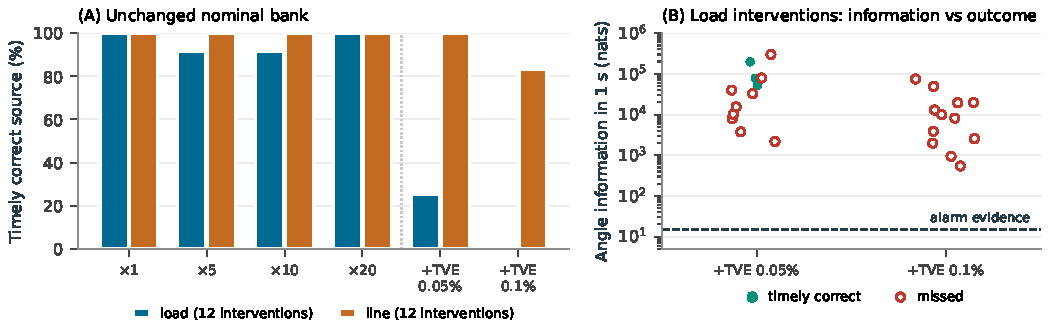
\includegraphics[width=.97\textwidth]{figures/generated/noise_stress.pdf}
\caption{Nominal bank under increased PMU noise, with fixed publication rules and widened startup noise-scale support. (A) Timely attribution under uniform noise scaling and added independent noise, with component standard deviation $\sigma$ (relative magnitude and radian angle). (B) One-second matched-signature energy using only the added independent angle noise, against the observed outcome. The dashed line is an idealized score reference, not the bank's publication threshold.}
\label{fig:noise-stress}\end{figure*}

\begin{table}[h]\centering\small
\caption{Noise-stress outcomes with fixed publication thresholds and widened startup noise-scale support. $\sigma$ is the standard deviation of each added relative-magnitude and radian-angle component.}
\label{tab:noise-stress}
\begin{tabular}{@{}lrrrr@{}}\toprule
Scenario & Load & Line & Extras & Normal\\\midrule
$\times1$ & \RevNoiseOneLoad & \RevNoiseOneLine & \RevNoiseOneExtras & \RevNoiseOneNormalFA\\
$\times5$ & \RevNoiseFiveLoad & \RevNoiseFiveLine & \RevNoiseFiveExtras & \RevNoiseFiveNormalFA\\
$\times10$ & \RevNoiseTenLoad & \RevNoiseTenLine & \RevNoiseTenExtras & \RevNoiseTenNormalFA\\
$\times20$ & \RevNoiseTwentyLoad & \RevNoiseTwentyLine & \RevNoiseTwentyExtras & \RevNoiseTwentyNormalFA\\
$\sigma=0.0005$ & \RevNoiseTVEaLoad & \RevNoiseTVEaLine & \RevNoiseTVEaExtras & \RevNoiseTVEaNormalFA\\
$\sigma=0.001$ & \RevNoiseTVEbLoad & \RevNoiseTVEbLine & \RevNoiseTVEbExtras & \RevNoiseTVEbNormalFA\\\bottomrule
\end{tabular}\end{table}
